% !TEX encoding = UTF-8 Unicode

\Chapter{Művészi jellegű szűrők}

A mai világban elég népszerűek az olyan számítógépes vagy mobiltelefonos alkalmazások, amelyekkel fényképeket vagy videókat lehet átalakítani valós időben, képfeldolgozási módszerekkel. Dolgozatomban ezen alkalmazások működésének hátterével, jellemző algoritmusaival és megvalósítási módjukkal foglalkozom.

A művészi szűrők mögött komoly tudományos eredmények állnak. Többen foglalkoznak azzal, hogy egy-egy művészi jellegű hatás megvalósításának milyen lehetőségei vannak. Alapvetően nagyon irányzatként a témakörben az élek megtartásával történő szűrést \cite{artistic}, és a szegmentálásra épülő objektumkijelölést \cite{intellipaint} különíthetjük el.

A következő szakaszok egyelőre azt vizsgálják, hogy milyen területeken találkozhatunk a művészi szűrők alkalmazásával a népszerű weboldalak és alkalmazások körében.

\Section{Népszerű alkalmazási területek}

A fiatalok többsége ha képfeldolgozásról van szó egyből a közösségi média adta lehetőségekre gondol. Ilyen például az Instagram, Snapchat vagy a Messenger alkalmazások. Ezek az applikációk a telefonok, tabletek kameráját használja, mint a képek vagy videók forrását. Dolgozatomban ezek működésére is kitérek.

\SubSection{Közösségi alkalmazások}

A közösségi alkalmazásokba előszeretettel építenek különféle képfeldolgozási módszereket. \Aref{fig:social_media}. ábrán láthatunk egy-egy példát az Instagram, Snapchat és Messenger alkalmazások egy-egy szűrőjének alkalmazására. A következőkben ezen alkalmazások rövid áttekintésére kerül sor.

\paragraph{Instagram} 

Valószínűleg az Instagram egyik legismertebb applikáció, amely képekkel és képfeldolgozással foglalkozik \cite{instagram}. Ez az alkalmazás pontosan arra készült, hogy a felhasználók megoszthassák egymással  ezeket, majd különféle művészi szűrőkkel láthassanak el. A szűrők köre folyamatosan bővül, valamit egyre testreszabhatók lesznek, például lehet állítani a képek dőlésszögén, fényességén, hogy mennyire legyen kontrasztos, a színek melegségén, mennyire legyen elmosva és hogy hol legyenek az elmosódások.

\paragraph{Snapchat} 

A Snapchat is egy képfeldolgozással kapcsolatos alkalmazás \cite{snapchat}, bár teljesen más a koncepció mint az Instagram esetében. Itt is a barátainkkal, imerőseinkkel tudjuk megosztani a grafikus tartalmainkat, de ezek a nyilvánosság számára nem láthatók, csak azok láthatják akiknek adunk jogosultságot, hogy láthassák és ők is csak egy bizonyos ideig, amit mi határozunk meg küldéskor. Ez az alkalmazás nem csak egyszerűen művészi szűrőkkel foglalkozik, hanem képes detektálni az arcokat. Mivel az alkamazás felismeri az arcunkat, így különböző tárgyakat/effekteket képes rárakni ennek megfelelően, például napszemüveget, vicces sapkákat,  különböző fényeket, eltorzítja az arcunk vagy a szemünket.

\paragraph{Messenger} 

Ez az alkalmazás nem kifejezetten képfeldolgozással foglalkozik, azonban már megjelentek benne ezek a funkciók is. Ebben az alkalmazásban barátainkkal, imerőseinkkel tudunk chatelni, tartalmakat megosztani, akár privát módon, akár csoportosan \cite{messenger}. Képeinket hasonló módon tudjuk szerkeszteni, mint a Snapchat alkalmazással. Itt is arcfelismerés alapján tud rárakni az arcunkra a program mindenféle effektet. Ebben a programban elérhető a videóhívás is ahol szintén haszálhatók effektek.

\begin{figure}[ht]
\centering
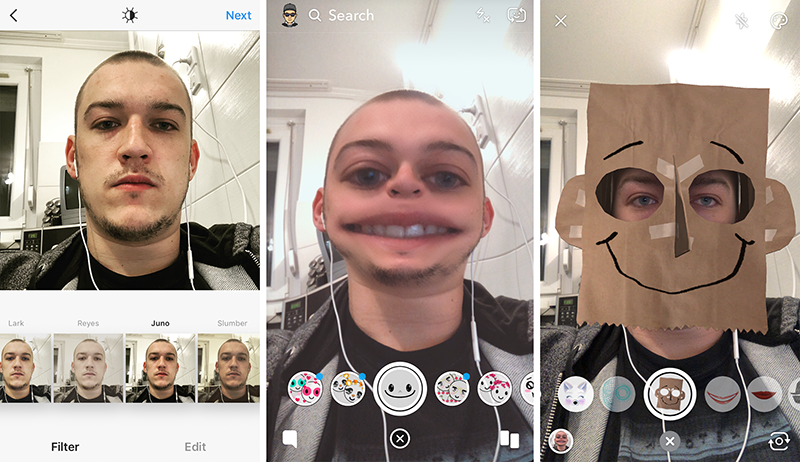
\epsfig{file=kepek/instasnapmess.png,scale=0.47}
\caption{Az Instagram, Snapchat és Messenger alkalmazások művészi szűrőiről készült képernyőfotók} 
\label{fig:social_media}
\end{figure}

\SubSection{Webkamera- és mobil alkalmazások}

A közösségi alkamazásokon kívül, van néhány olyan weboldal, mobil alkalmazás amely szintén komplikáltabb képfeldolgozási módszereket használ. A következőkben ezek közül a Prisma alkalmazást és a webkamerás alkalmazások néhány jellemzőjét mutatom be.

\paragraph{Prisma}

Ez az alkalmazás a képfeldolgozáshoz mesterséges intelligenciát, jellemzően neurális hálókat haszánál, hogy művészi szűrőkkel ellátott képeket hozzon létre \cite{prisma}. A felhasználó az alkalmazásba betölti az átalakítandó fényképet, kiválasztja a számára megfelelő szűrőt, pár másodperc múlva a szűrővel elláttott kép megjelenik az alkalmazásban. A képfeldolgozás a Prisma esetében távoli szerveren történik.

\paragraph{Webkamera alkalmazások} 

Számtalan olyan program, webalkalmazás van amely tartalmaz képfeldolgozási funkciókat. Egy ilyen például a \textit{Pixect} \cite{pixect}. Léteznek továbbá gyári beépített programok, amelyek a webkamera saját illesztőprogramjában találhatók meg, és különböző szűrőket tudnak rárakni a képekre. Művészi szűrőkkel ellátott képekre láthatunk néhány példát \aref{fig:prisma}. ábrán.

\begin{figure}[ht]
\centering
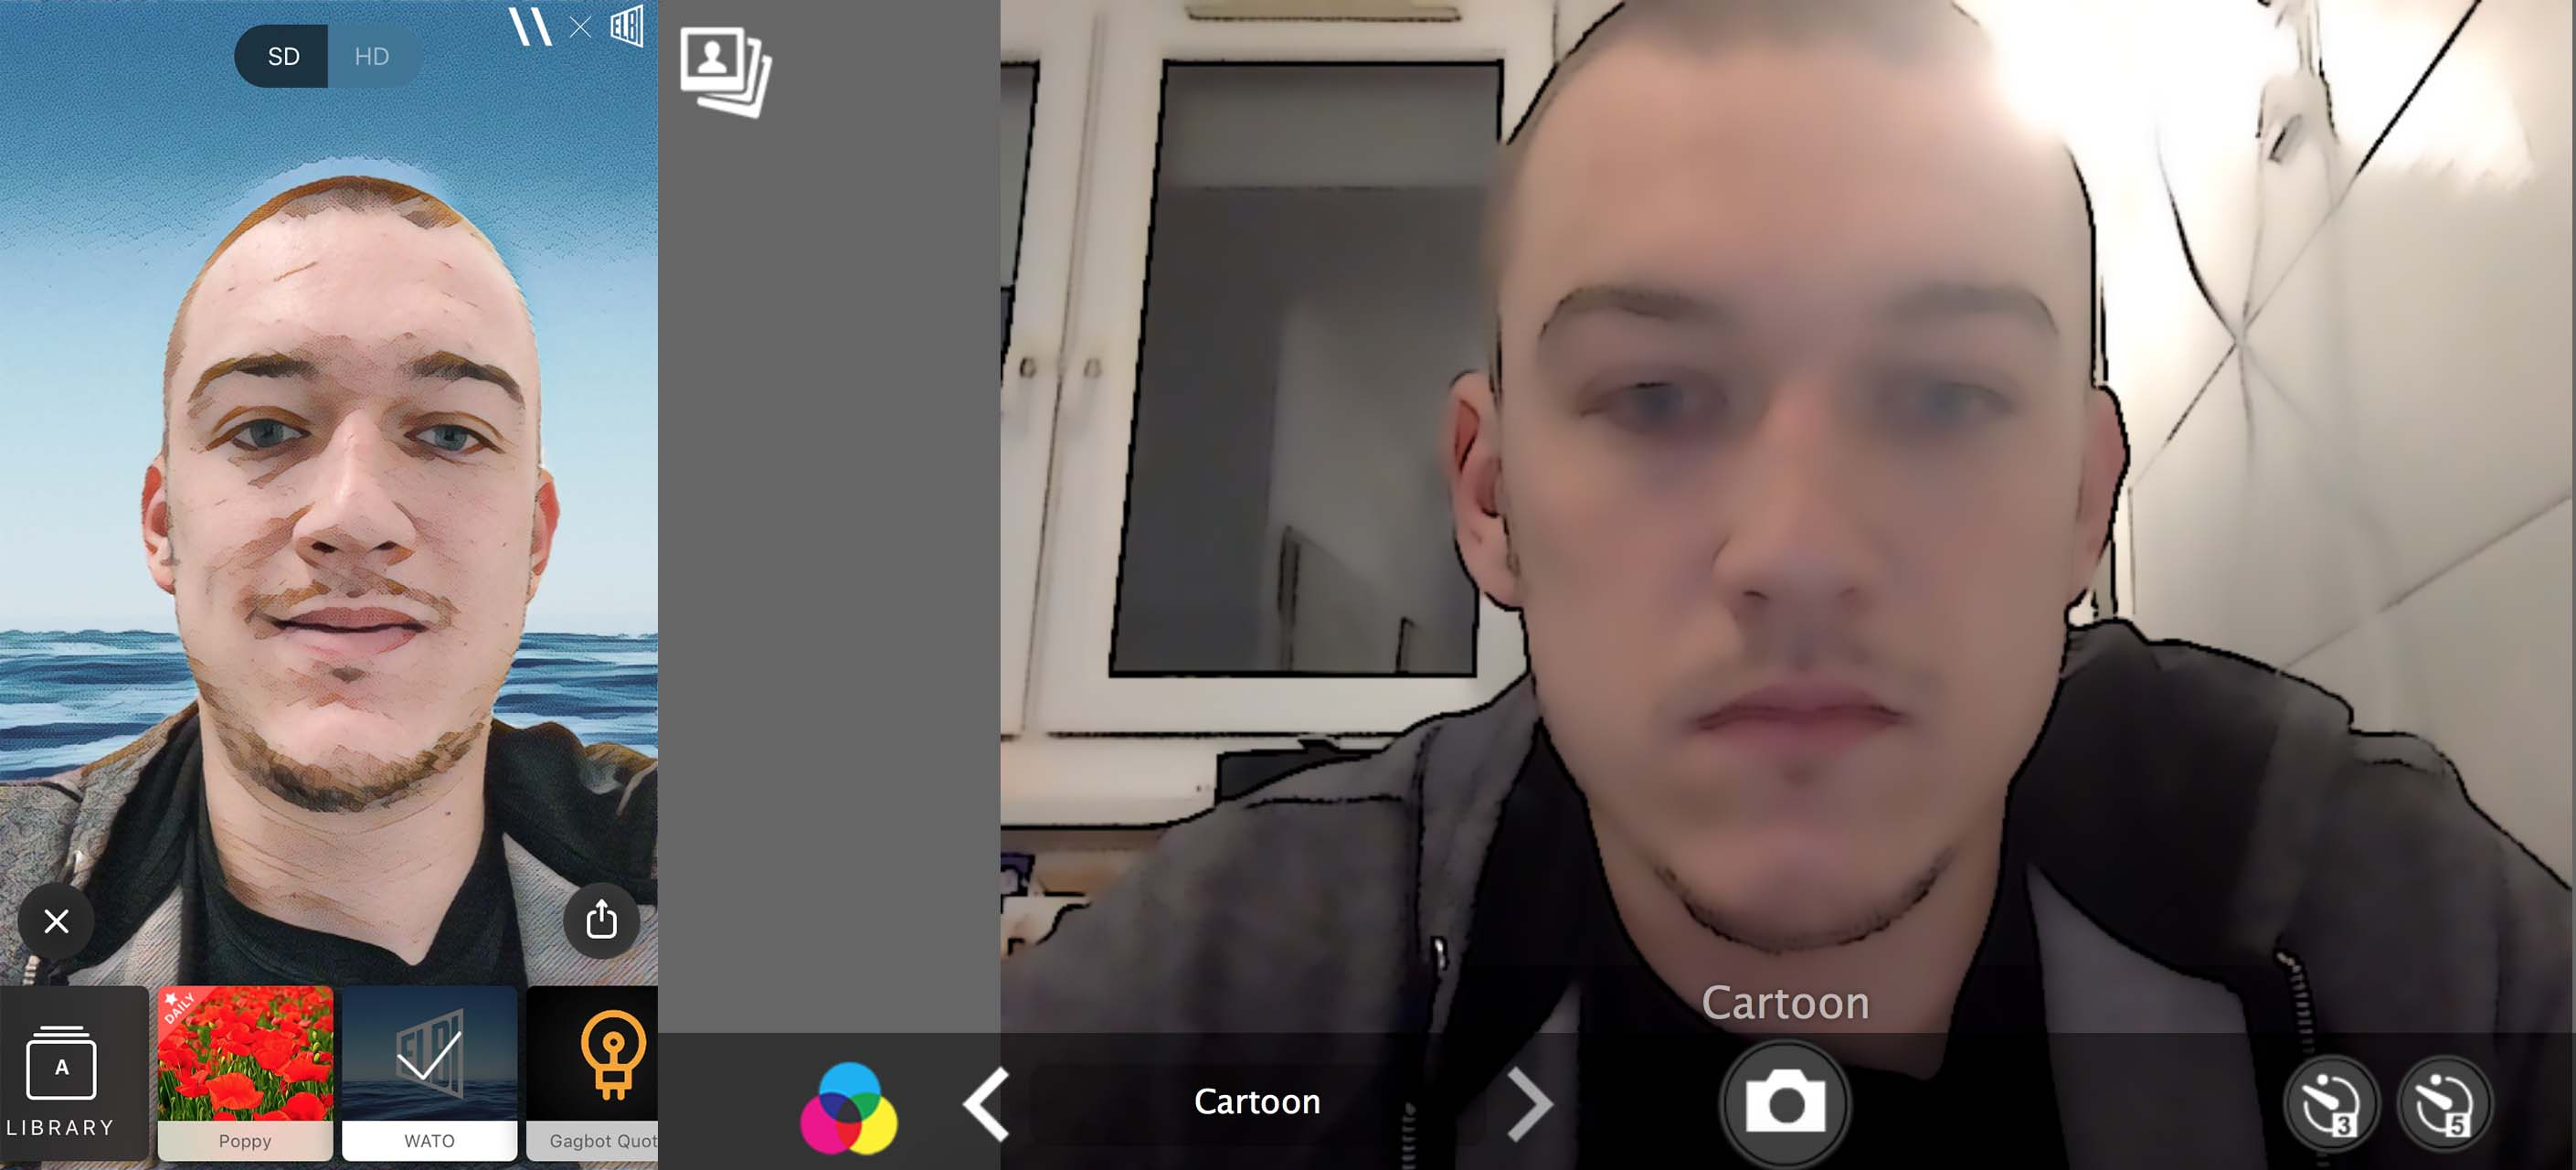
\epsfig{file=kepek/prismawebcam.jpg,scale=0.3}
\caption{Példa a Prisma és a \texttt{https://www.pixect.com} alkalmazások által készített művészi szűrőkkel ellátott képekre.} 
\label{fig:prisma}
\end{figure}

\SubSection{Filmek, játékok amelyekhez művészi szűrőket használtak}

Művészi jellegű szűrőket nem csak magánfelhasználók használnak arra, hogy érdekesebbé tegyék az elkészült fényképeiket, videóikat, hanem ilyen filtereket használnak videójátékok és filmek esetében is. Nézzünk meg ezekre is néhány példát!

\paragraph{Jet Set Radio videójáték} 

A \textit{Jet Set Radio} volt a világon az első olyan videójáték amelyen sötét árnyalatú grafikákat mutattak be, túlzott alakokkal, vastag vonalakkal és lapos, élénk színekkel \cite{jetset}. Ezzel olyan érzetet keltve, mint ha egy képregény vagy egy rajzfilm lenne. A játékban egy görkorcsolyázó karaktert lehet irányítani és graffitiznie kell a megadott helyekre mielőtt lejár az idő. Plusz pontokért lehet mindenféle extrém trükköt is csinálni korcsolyázás közben. Nehezítésként a játékost üldözik gyalogosan, helikopterekkel és tankokkal.

\paragraph{Kamera által homályosan (A Scanner Darkly) című film} 

A \textit{Kamera által homályosan} című filmet digitálisan forgatták, majd interpolált rotoszkóp segítségével animálták \cite{scannerdarkly}\cite{porthu}. Ez egy olyan animációs technika, melyben az eredeti felvételekből képkockáról képkockára filtereztek. Ezzel olyan hatást értek el, hogy azt lehet mondani erre a filmre, hogy animációs film. A film a közeljövőben játszódik. A lakosság nagy része drog fogyasztó. Beépített titkos ügynökökkel és különböző megfigyelési rendszerekkel próbálnak rendet tartani. Az egyik detektívnek, Frednek kiadják parancsba, hogy álljon rá egy nagyon veszélyes kábítószert terjesztőre, Bob Arctor-ra. A drog hatása az, hogy az emberek személyisége két, egymással ellentétes felére bomlik. Kiderül, hogy Arctor igazából Fred alteregója, igy ez az ügy elég nagy kihívásokkal jár. 
% Port.hu irodalom jegyzék 

Az említett videójátékról és filmről \aref{fig:jetset}. ábrán láthatunk egy-egy képet.

\begin{figure}[ht]
\centering
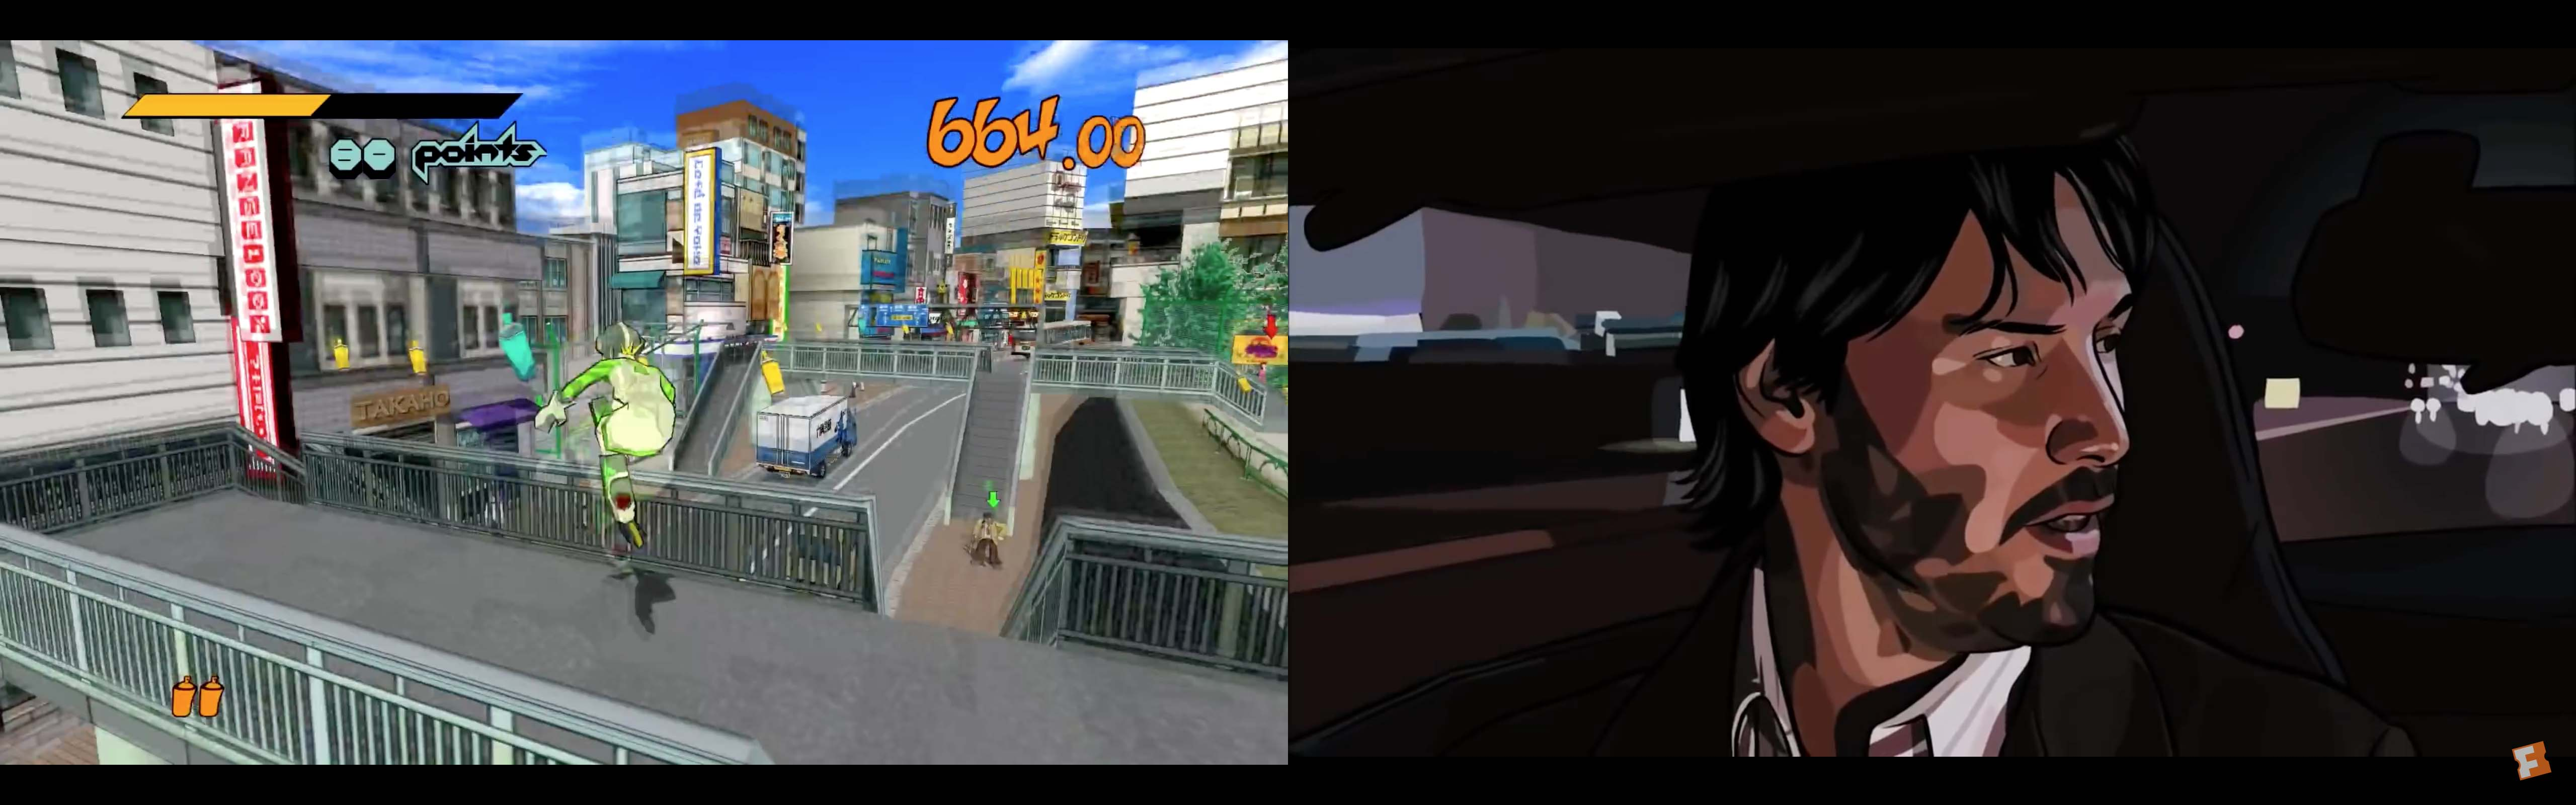
\epsfig{file=kepek/jatekfilm,scale=0.17}
\caption{Jet Set Radio videójáték és Kamera által homályosan c. film egy-egy jellegzetes képkockája} 
\label{fig:jetset}
\end{figure}

\Section{A megvalósítás nehézségei}

A digitális képfeldolgozás számítógépes algoritmusokat használ a digitális képek készítéséhez. Ez lehetővé teszi, hogy sokkal szélesebb körű algoritmusokat alkalmazzanak a bemeneti adatokra, és ezekkel az algoritmusokkal elkerülhetők az olyan problémák, mint a zaj és a jelek torzulása a feldolgozás során. Mivel a képeket két dimenzióban definiálják, a digitális képfeldolgozást multidimenzionális rendszerek formájában lehet modellezni.  Ezekkel a képfeldolgozási algoritmusokkal lehet olyan képeket készíteni, amiket például azok az alkamazások is létrehoznak amiket ebben a fejezetben bemutattam.

%https://en.wikipedia.org/wiki/Digital_image_processing

\Section{Elvárások a szűrőkkel kapcsolatban}

Olyan szűrőket szeretnék létrehozni, amelyek hasonlóképpen működnek, mint azok az applikációk, játékok, filmek amelyeket ebben a fejezetben említettem. Rajzfilm (\textit{cartoon}) jellegű, festmény szerű, valamint ceruza rajz jellegű szűrőket szándékozok létrehozni, amelyeket képekre, videókra lehet alkalmazni. A dolgozatomban ezek számítási idejét tesztelni is fogom.
